\documentclass[aspectratio=169,
   %handout
]{beamer}

%\usepackage{pgfpages}
%\pgfpagesuselayout{2 on 1}[a4paper, border shrink=8mm]
%\setbeameroption{show notes on second screen=bottom}
%\pgfpageslogicalpageoptions{1}{border code=\pgfusepath{stroke}}

\usetheme{metropolis}
\setbeamercovered{transparent}
\setbeamertemplate{navigation symbols}{}

\bibliographystyle{alpha}

\definecolor{unibsblue}{RGB}{60, 88, 155}
\definecolor{lightbeige}{RGB}{255, 251, 241}
\definecolor{textcolor}{RGB}{50, 50, 50}

\usepackage{cmbright}
\usepackage{subfig}
\usepackage{appendixnumberbeamer}
\usepackage{siunitx}
\usepackage[final]{graphicx}
\usepackage{pdfpages}

\graphicspath{{images}}
\usepackage[main=italian,english]{babel}
\usepackage[utf8]{inputenc}
\usepackage{csquotes}
\usepackage[T1]{fontenc}
\usepackage{hyphenat}

%\bibliographystyle{plain}
%\renewcommand{\bibname}{Bibliografia e Sitografia}

\usepackage[backend=biber,doi=false,isbn=false,mincitenames=1,maxcitenames=4,style=ieee]{biblatex}
\DeclareFieldFormat{sentencecase}{#1} % never apply sentence casing, even if bibtex field is unprotected
\DeclareFieldFormat{titlecase}{#1} % never apply title casing, even if bibtex field is unprotected
\addbibresource{./biblio/datasheets.bib}
\addbibresource{./biblio/refs.bib}
\addbibresource{./biblio/sites.bib}
\addbibresource{./biblio/images.bib}


\title[Relazione Finale]{Sviluppo di un sistema di supporto alla programmazione per dispositivi integrati della famiglia AVR}
\author[S.Fontana --- 727199]{Stefano Fontana}
\date{2021/2022}
\makeatletter 
    \newcommand{\insertrawshotauthor}{\beamer@shortauthor} 
    \newcommand{\insertrawshorttitle}{\beamer@shorttitle} 
    \setlength{\metropolis@frametitle@padding}{3.5ex}% <- default 2.2 ex
\makeatother

\defbeamertemplate*{title page}{customized}[1][]
{
    \begin{center}
        
\includegraphics[width=.23\textwidth]{logo_unibs_40.png}

        DIPARTIMENTO DI INGEGNERIA DELL'INFORMAZIONE
        
        Corso di Laurea in Ingegneria Informatica
    \end{center}
    \vfill
    \begin{center}
        {\fontfamily{cmr}\fontsize{14}{27}\color{black}\selectfont\textbf{\inserttitle}}
    \end{center}
    \vfill
    \begin{minipage}{.48\textwidth}
        \textbf{Relatore:}\\
        Chiar.mo~Prof.~Alessandro~Depari
    \end{minipage}
    \begin{minipage}{.5\textwidth}
        \begin{flushright}
            \textbf{Laureando:}\\
            \insertauthor\\
            Matr. 727199
        \end{flushright}
    \end{minipage}
    \begin{center}
        Anno Accademico \insertdate
    \end{center}
}
\setbeamertemplate{frametitle continuation}{\hfill\insertcontinuationcount}

\setbeamertemplate{footline}[text line]{%
    \parbox{.85\linewidth}{
        \vspace*{10mm}
        {\color{unibsblue}\par\noindent\rule{\linewidth}{0.1pt}}\\
        \insertrawshotauthor\hfill
        A.A. 2021/2022\hfill
        \insertframenumber/\inserttotalframenumber%
    }\hfill
    \parbox{.15\textwidth}{
        \vspace*{5mm}
        \hspace*{5mm}
        
\includegraphics[height=10mm]{logo_unibs_40.png}
    }
}
\setbeamertemplate{navigation symbols}{}

\setbeamercolor{background canvas}{bg=white}
\setbeamercolor{normal text}{fg=textcolor}
\setbeamercolor{frametitle}{bg=unibsblue, fg=white}

\hypersetup{
    pdftitle={Sviluppo di un sistema di supporto alla programmazione per dispositivi integrati della famiglia AVR - Presentazione},
    pdfsubject={PresentazioneRelazioneFinale},
    pdfauthor={Stefano Fontana},
    hidelinks
}

\newlength{\parskipbackup}
\setlength{\parskipbackup}{\parskip}
\newlength{\parindentbackup}
\setlength{\parindentbackup}{\parindent}
\newcommand{\baselinestretchbackup}{\baselinestretch}

\usetemplatenote{\rmfamily%
  \setlength{\parindent}{1em} \setlength{\parskip}{1ex}%
  \renewcommand{\baselinestretch}{1}%
  \noindent \insertnote%

  \setlength{\parskip}{\parskipbackup}%
  \setlength{\parindent}{\parindentbackup}%
  \renewcommand{\baselinestretch}{\baselinestretchbackup}%
}

\begin{document}

    \pagenumbering{gobble}
    \maketitle
    \note{Ringrazio il presidente per l'introduzione.\\Presenterò ora un elaborato sullo sviluppo si un sistema di debug per microcontrollori}

    \begin{frame}
        \frametitle{Contesto \hfill 1}
    
        La programmazione di microcontrollori è una pratica complessa:

        \begin{minipage}{.65\textwidth}
            \begin{itemize}
                \item <1-> Programmazione a basso livello
                \item <2-> Set di istruzioni specifici e poco conosciuti
                \item <3-> Complessi flussi di codice, interrupt, esecuzioni in tempo reale
                %\item <4-> Strumenti e software proprietari e costosi
            \end{itemize}
        \end{minipage}
        \begin{minipage}{.34\textwidth}
            \begin{figure}
                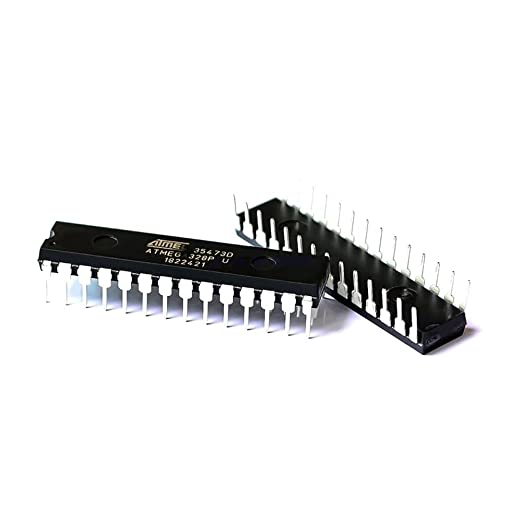
\includegraphics[width=\textwidth]{atmega328.jpg}
            \end{figure}
        \end{minipage}    

        \note<1>[]{
            Programmazione C e assembly a basso livello
        }

        \note<2>[]{
            In genere set di istruzioni specifici per la famiglia e poco conosciuti
        }

        \note<3>[]{
            La gestione logica degli interrupt è complessa e richiede profonde conoscenze dell'architettura. Inoltre si aggiunge complessità per via di questioni di tempo di esecuzione delle routine di interrupt.
        }
    \end{frame}


    \begin{frame}
        \frametitle{Contesto \hfill 2}

        \begin{minipage}{.6\textwidth}
            Sono disponibili strumenti per facilitare la programmazione
            \begin{itemize}
                \item <1-> Strumenti interattivi di analisi del flusso di esecuzione (\textit{debugger})
                \item <2-> Ambienti di sviluppo avanzati
                \item <3-> Tipicamente hardware e software proprietari
                \begin{itemize}
                    \item <4-> Compatibilità con sistemi operativi
                    \item <5-> Costo
                \end{itemize}
            \end{itemize}
        \end{minipage}
        \begin{minipage}{.38\textwidth}
            \begin{figure}
                \includegraphics<1|handout:0>[width=\textwidth]{vscode-dbg-decoration.png}
                \includegraphics<2-4|handout:0>[width=\textwidth]{atmelstudio.png}
                \includegraphics<5>[width=\textwidth]{avrisp.png}
            \end{figure}
        \end{minipage}

        \note<1->[]{
            Esistono software in grado di facilitare la programmazione in questo ambito. Essi sono in grado di fornire assistenza allo sviluppatore agevolando operazioni ripetitive e analizzando il flusso del codice preventivamente.

            In genere sono software proprietari e spesso sono compatibili con uno specifico sistema operativo, oltre che spesso fanno uso di dispositivi per interfacciarsi con il target che possono essere costosi.
        }

    \end{frame}

    \begin{frame}
        \frametitle{Obiettivi}
        
        Sviluppo di un insieme di strumenti per il debugging
        \begin{itemize}
            \item <1-> \textbf{Open Source}
            \item <2-> \textit{Debugging} con limitato impiego di risorse
            \item <3-> Facilità d'uso
            \item <4-> Compatibilità del software su piattaforme multiple (Windows, MacOS, Linux)
        \end{itemize}

        \note<1->[]{
            Gli obiettivi dell'elaborato consistono nello sviluppo di una serie di strumenti per l'assistenza alla programmazione tali che siano open source, permettano il debugging limitando l'impiego di risorse del target, siano semplici da utilizzare e configurare e siano compatibili con una vasta gamma di piattaforme.
        }
    \end{frame}

    %\begin{frame}
    %    \frametitle{Stato dell'arte}
    %    La programmazione di microcontrollori viene effettuata tramite tre macro passaggi
    %    \begin{enumerate}
    %        \item<1-> Codifica $\rightarrow$
    %        {\footnotesize Il codice viene scritto dal programmatore e compilato in formato binario}
    %        \item<2-> Caricamento $\rightarrow$
    %        {\footnotesize Il programma viene scritto sulla memoria del controllore tramite l'uso di un programmatore}
    %        \item<3-> Esecuzione $\rightarrow$
    %        {\footnotesize Il controllore viene quindi avviato e il programma viene eseguito.}
    %    \end{enumerate}
%
    %    \begin{figure}
    %        \begin{tikzpicture}[scale=.8]
    %            \draw[fill=green!50] (0,0) rectangle (2,2) node[pos=.5] {\textit{host}};
    %            \draw[fill=yellow!50] (5,0.5) rectangle (8,1.5) node[pos=.5] {\textit{Programmer}};
    %            \draw[fill=blue!50] (11,0.5) rectangle (12.5,1.5) node[pos=.5] {\textit{target}};
    %            \node (0) at (1, -0.5) {1. Codifica};
    %            \node (0) at (6.5, -0.5) {2.Caricamento};
    %            \node (0) at (11.75, -0.5) {3. Esecuzione};
    %            \draw [stealth-stealth](2,1) -- (5,1) node[label={[font=\footnotesize]above:USB},pos=.5] {};
    %            \draw [stealth-stealth](8,1) -- (11,1) node[label={[font=\footnotesize]above:SPI/JTAG\cite{avr:appnote:isp}},pos=.5] {};
    %        \end{tikzpicture}
    %    \end{figure}
    %\end{frame}
    %\note{
    %    Il programmatore converte un protocollo complesso (USB/seriale) in comandi adatti alla programmazione dell'integrato su bus parallelo/spi
    %}

    \begin{frame}
        \frametitle{Famiglia AVR}
        La famiglia AVR di Atmel --- Ad oggi Microchip ---
        \begin{itemize}
            \item<1-> Comprende microcontrollori a 8bit \SI{20}{\mega\hertz} 20 MIPS
            \item<2-> Programmazione ``in system'' (ISP) tramite interfaccia seriale sincrona
            \item<3-> {\color{red} Protocollo di debug proprietario (debugWire) non ufficialmente documentato}
            \item<4-> {\color{red} Ambiente di sviluppo freeware ma mono-piattaforma (Windows)}
        \end{itemize}

        \begin{figure}
            \begin{tikzpicture}[scale=.8]
                \draw<5>[fill=green!50] (-2,0) rectangle (1,2) node[pos=.5] {\textit{Atmel Studio}};
                \draw<5>[fill=yellow!50] (4,0) rectangle (9,2) node[pos=.5] {\textit{Programmer/Debugger}};
                \draw<5>[fill=blue!50] (12,0.5) rectangle (13.5,1.5) node[pos=.5] {\textit{AVR}};
                \node<5> (0) at (-0.5, -0.5) {Host};
                \node<5> (0) at (12.75, -0.5) {Target};
                \draw<5> [stealth-stealth](1,1) -- (4,1) node[label={[font=\footnotesize]above:USB},pos=.5] {};
                \draw<5> [stealth-stealth](9,0.6) -- (12,0.6) node[label={[font=\footnotesize]below:ISP},pos=.5] {};
                \draw<5> [stealth-stealth](9,1.2) -- (12,1.2) node[label={[font=\footnotesize]above:DebugWire},pos=.5] {};
            \end{tikzpicture}
        \end{figure}

        \note<1->[]{
            Gli obiettivi di questo elaborato sono stati applicati alla famiglia AVR di atmel.
            
            È una famiglia di controllori a 8 bit e 20 milioni di istruzioni al secondo, in grado di essere riprogrammata nel circuito di destinazione (ISP). Possiede anche una periferica di debug in hardware ma il protocollo di comunicazione è proprietario e non ufficialmente documentato.
            Lo sviluppo per questa piattaforma avviene grazie ad Atmel Studio, software freeware ma non disponibile su tutti i sistemi operativi.
        }
    \end{frame}

    \begin{frame}
        \frametitle{Target}
        \textbf{Arduino UNO R3}
        
        ATMega328P-PU {\footnotesize Processore a 8 bit, \SI{20}{MIPS}, \SI{20}{\mega\hertz}@\SI{5}{\volt}}

        \begin{itemize}
            \item<1-> Non è presente il programmatore
            \item[] <2-> \(\Rightarrow\) Programmazione tramite convertitore USB-RS232 + bootloader
            \item[] <3-> \(\Rightarrow\) Perdita di una porzione della memoria flash
            \item <4-> Non è implementato il debugger
            \item[] <5-> \(\Rightarrow\) Solo Monitor Debugger Software \(\Rightarrow\) Perdita dell'unica seriale hardware
        \end{itemize}

        \begin{figure}
            \footnotesize
            \begin{tikzpicture}[scale=.65]
                \draw[fill=green!50] (-2,0) rectangle (1,2) node[pos=.5] {\textit{Arduino IDE}};
                \draw[fill=yellow!50] (4,0) rectangle (9,2) node[pos=.5] {\textit{USB - RS232}};
                \draw[fill=blue!50] (12,0) rectangle (14.5,1) node[pos=.5] {\textit{User PGM}};
                \draw[fill=blue!50] (12,1) rectangle (14.5,2) node[pos=.5] {\textit{bootloader}};
                
                \draw [stealth-stealth](1,1) -- (4,1) node[label={[font=\footnotesize]above:USB},pos=.5] {};
                \draw [stealth-stealth](9,1) -- (12,1) node[label={[font=\footnotesize]above:RS232},pos=.5] {};
                \node (0) at (-0.5, 2.5) {\textit{host}};
                \node (0) at (13.25, 2.5) {\textit{target}};
            \end{tikzpicture}
        \end{figure}

        \note<1->[]{
            L'hardware scelto per sviluppare l'elaborato è la scheda Arduino UNO R3, scelta per la grande diffusione e il supporto della community open source, oltre alla grande disponibilità di librerie.

            Essa monta un ATMega328P.

            Per motivi di costo, la scheda non fa uso di un programmatore dedicato bensì viene programmata grazie a un bootloader presente nella memoria flash del target e con il quale si interagisce grazie a un convertitore USB-Seriale.
            Questo implica che parte della memoria flash sia dedicata al bootloader e non sia utilizzabile.

            Inoltre, sempre per motivi di costi, non è stato implementato il debugger. Risulta quindi necessario praticare il monitor debugging inviando messaggi tramite la periferica UART del dispositivo rinunciandone all'utilizzo.
        }
    \end{frame}
        

    \begin{frame}
        \frametitle{Architettura Gnu Debugger (GDB)}
    
        \begin{itemize}
            \item[] <1-> GDB è una suite di software di \textit{debugging} multi-architettura open source
            \item[] <2-> Permette di lavorare su un processo remoto tramite l'architettura client-server
            %\item[] <3-> Server GDB sul programmatore $\rightarrow$ {\footnotesize Converte i comandi del client nelle controparti del protocollo di debug}
        \end{itemize}
        \begin{figure}
            \begin{tikzpicture}
                \draw[fill=green!50] (0,0) rectangle (2,2) node[pos=.5] {Client};
                \draw[fill=yellow!50] (5,0.5) rectangle (7,1.5) node[pos=.5] {Server};
                \draw[fill=purple!50] (7,0.5) rectangle (8,1.5) node[pos=.5] {Conv};
                %\draw[fill=red!50] (10.3,0.5) rectangle (11,1.5) node[pos=.5] {\small dW};
                \draw[fill=blue!50] (10.3,0.5) rectangle (12.5,1.5) node[pos=.5] {\textit{target}};

                \draw [stealth-stealth](2,1) -- (5,1) node[label={[font=\footnotesize]above:Protocollo GDB},pos=.5] {};
                \draw [stealth-stealth](8,1) -- (10.3,1) node[label={[font=\footnotesize]above:Debug},pos=.5] {};
                \draw [stealth-stealth](8,1) -- (10.3,1) node[label={[font=\footnotesize]below:Protocol},pos=.5] {};

                %\draw (4.8, 0) rectangle (11.2, 2);
                %\node (0) at (8, 2.5) {Ambito di sviluppo};
            \end{tikzpicture}
        \end{figure}
        \note<1->{
            Al fine di implementare le funzionalità di debugging, si è deciso di utilizzare ``Gnu Debugger'' in quanto permetta un'architettura client-server. Grazie a ciò è possibile implementare il server GDB, software in grado di comprendere i comandi a basso livello del client per poi tradurli in comandi debugWire, su un microcontrollore con la capacità di interagire con il target.
        }
    \end{frame}
    

    \begin{frame}
        \frametitle{Implementazione}
    
        \begin{figure}
            \begin{tikzpicture}[scale=.7]
                \node[inner sep=0pt] (arduino) at (0,0) {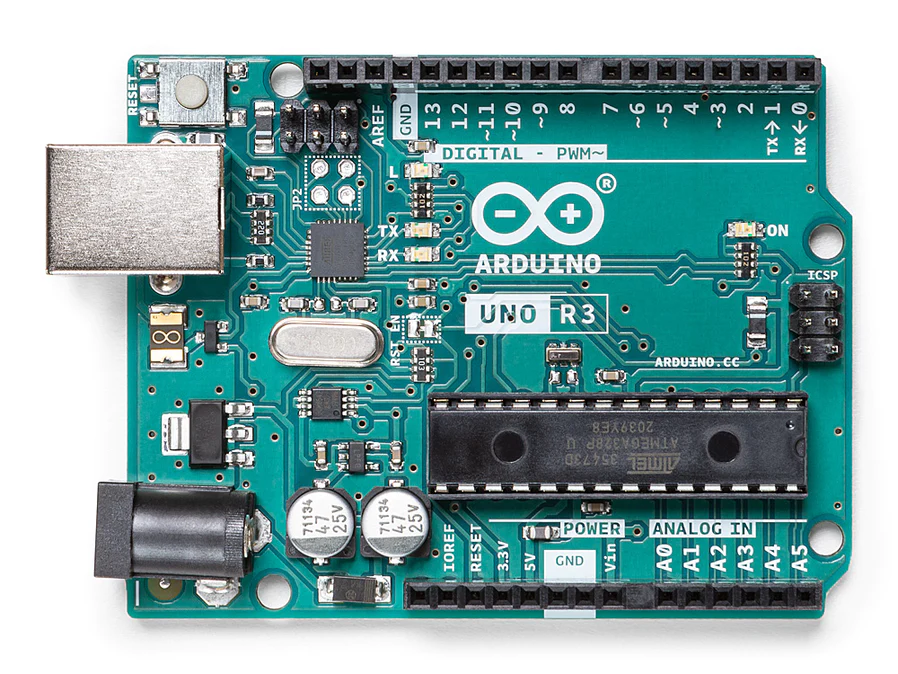
\includegraphics[width=.35\textwidth]{arduino-no-annotations.png}};

                \draw [fill=green!50] (-8, 0) rectangle (-6, 2) node [pos=.5] {Host};
                \draw [fill=yellow!50] (-1.1, 0.45) rectangle (-0.65, 0.88) node [pos=.5] {A};
                \draw [fill=blue!50] (2.75, -0.55) rectangle (-0.15, -1.15) node [pos=.5] {Target};

                \draw [semithick] (-6, 1) -- (-3.1, 1) node[pos=.5, label={above:USB}] {};
                \draw [color=yellow, thick] (-1.8, 1) -- (-1.45, 1) -- (-1.235, 0.665) -- (-1.1, 0.665);
                \draw [color=red, thick] (-0.65, 0.665) -- (2.3, 0.665) -- (2.5, 0.465) -- (2.5, -0.3) -- (2.7, -0.5);
            \end{tikzpicture}
        \end{figure}

        La scheda Arduino implementa la comunicazione \textit{target-host} mediante un microcontrollore (ATMega16U2)\pause

        È stato sviluppato un server GDB e l'adattatore per debugWire sull'ATMega16U2 presente sulla scheda Arduino.
        \note<1->[]{
            La scheda Arduino UNO implementa il convertitore USB-Seriale tramite un controllore (ATMega16U2) dedicato alla commutazione tra USB-CDC e uart. Inoltre il controllore gestisce il pin di reset del target.

            Tale controllore è stato usato per sviluppare il firmware che permette la conversione tra protocollo GDB e debugWire.
        }
    \end{frame}

    \begin{frame}
        \frametitle{Implementazione - Architettura}
    
        Server GDB sul convertitore $\rightarrow$ {\footnotesize Converte i comandi del client nelle controparti del protocollo debugWire}

        \begin{figure}
            \begin{tikzpicture}
                \draw[fill=green!50] (0,0) rectangle (2,2) node[pos=.5] {Client};
                \draw[fill=yellow!50] (5,0.5) rectangle (7,1.5) node[pos=.5] {Server};
                \draw[fill=purple!50] (7,0.5) rectangle (8,1.5) node[pos=.5] {Conv};
                \draw[fill=red!50] (10.3,0.5) rectangle (11,1.5) node[pos=.5] {\small dW};
                \draw[fill=blue!50] (11,0.5) rectangle (12.5,1.5) node[pos=.5] {\textit{target}};

                \draw [stealth-stealth](2,1) -- (5,1) node[label={[font=\footnotesize]above:Protocollo GDB},pos=.5] {};
                \draw [stealth-stealth](8,1) -- (10.3,1) node[label={[font=\footnotesize]above:debugWire},pos=.5] {};

                \draw (4.8, 0) rectangle (12.7, 2);
                \node (0) at (8.75, 2.5) {Arduino UNO R3};

                \node (1) at (6.5, 1.7) {\small ATMega16U2};
                \node (2) at (11.4, 1.7) {\small ATMega328P};
                \node (2) at (1, 2.5) {\small Visual Studio Code};
            \end{tikzpicture}
        \end{figure}

        \note<1->{
            È possibile vedere dalla figura come il server GDB e il target risiedano sulla scheda Arduino UNO. Il firmware installato sull'ATMega16U2 si occuperà di convertire i comandi del client, integrato nell'ide Visual Studio Code, in comandi debugWire validi.
        }
    \end{frame}

    \begin{frame}
        \frametitle{DebugWire}
    
        \begin{itemize}
            \item[]<1-> È il protocollo di debug di ATMega328P
            \item[]<2-> Sono pubblicamente disponibili definizioni parziali non ufficiali dei comandi principali
            \item[]<3-> Sostituisce la funzionalità di reset
            \item[]<4-> Protocollo fisico UART, half-duplex, one-wire open drain
        \end{itemize}

        \note<1->{
            debugWire è il protocollo usato per il debugging dell'ATMega328P e più in generale per la famiglia AVR.
            Il protocollo non è ufficialmente documentato ma sono disponibili definizioni parziali non ufficiali dei comandi e del livello fisico grazie ad operazioni di reverse engineering.

            La comunicazione è basata su una linea UART one-wire open-drain half-duplex sul pin di reset, impedendo quindi la normale operazione, senza necessitare di un pin dedicato.
        }
    \end{frame}

    \begin{frame}
        \frametitle{Circuito di Reset \hfill 1}
        \begin{figure}
            \begin{circuitikz}[scale=.8, american]
                \draw (0, 0) node[label={[font=\footnotesize]left:PD7}] {}
                to[short, *-] (1, 0) [C=C5] to (2,0);
                \draw (2,0) to[short, -*] (5, 0) node[label={[font=\footnotesize]right:\(\overline{\text{RST}}/\text{dW}\)}] {};
                
                \draw [short, *-] (0.5,0) [R] to (0.5,-3);
                \draw [short, *-] (3,0) [R] to (3,2);
                \draw (4,0) to[short, *-] (4, 1)[D] to (4,2);

                \draw (3,0) [nopb={RESET BTN}] to (3, -3);
                
                \draw (3,2) to (3,2.5) to (3.5,2.5) to (3.5, 3);
                \draw (4,2) to (4,2.5) to (3.5,2.5);
                \draw (3,3) -- (4, 3) node[pos=.5, label=above:VCC] {};
                \draw (2.5,-3) -- (3.5, -3) node[pos=.5, label=below:GND] {};
                \draw (0,-3) -- (1, -3) node[pos=.5, label=below:GND] {};


                \draw<2-> [red] (1, -0.5) -- (2, 0.5);
                \draw<2-> [red] (1, 0.5) -- (2, -0.5);

                \draw<3-> [red] (2.75, -0.5) -- (3.25, -0.35);
                \draw<3-> [red] (2.75, -0.7) -- (3.25, -0.55);


                \draw<4-> [red] (0.25, -0.5) -- (0.75, -0.35);
                \draw<4-> [red] (0.25, -0.7) -- (0.75, -0.55);

                \draw<2-> [green, short, *-] (0.5, 0) to (0.5, 1.5) -- (2.5, 1.5) to[green, short, -*]  (2.5, 0);
                \draw (-1, -1) -- (0, -1) -- (0, 1) -- (-1, 1);
                
                \draw (-1.5, -1) -- (0, -1) -- (0, 1) -- (-1.5, 1);
                \node (0) at (-0.8, 1) [label={above:\textit{Converter}}] {};

                \draw (6.5, -1) -- (5, -1) -- (5, 1) -- (6.5, 1);
                \node (0) at (5.5, 1) [label={above:\textit{target}}] {};
            \end{circuitikz}
        \end{figure}        
        \note<1->{
            Al fine di utilizzare il protocollo debugWire è necessaria una connessione diretta ed esclusiva tra il pin del convertitore e il pin di reset del target.

            A tal fine risulta necessario rimuovere il condensatore C5 e ristabilire la connessione.

            Inoltre è necessario isolare il pulsante di reset, utilizzato per permettere all'utente il reset del controllore, in quanto non più funzionante.

            Infine è necessario isolare il resistore di pulldown in quanto andrebbe a creare un partitore di tensione.
        }
    \end{frame}

    \begin{frame}
        \frametitle{Circuito di Reset - Risultato}
        \begin{minipage}{.5\textwidth}
            \begin{figure}
                \begin{circuitikz}[scale=.65, american]
                    \draw (0, 0) node[label={[font=\footnotesize]left:PD7}] {}
                    to[short, *-] (1, 0) [C=C5] to (2,0);
                    \draw (2,0) to[short, -*] (5, 0) node[label={[font=\footnotesize]right:\(\overline{\text{RST}}/\text{dW}\)}] {};
                    
                    \draw [short, *-] (0.5,0) [R] to (0.5,-3);
                    \draw [short, *-] (3,0) [R] to (3,2);
                    \draw (4,0) to[short, *-] (4, 1)[D] to (4,2);
    
                    \draw (3,0) [nopb={RESET BTN}] to (3, -3);
                    
                    \draw (3,2) to (3,2.5) to (3.5,2.5) to (3.5, 3);
                    \draw (4,2) to (4,2.5) to (3.5,2.5);
                    \draw (3,3) -- (4, 3) node[pos=.5, label=above:VCC] {};
                    \draw (2.5,-3) -- (3.5, -3) node[pos=.5, label=below:GND] {};
                    \draw (0,-3) -- (1, -3) node[pos=.5, label=below:GND] {};
    
    
                    \draw[red] (1, -0.5) -- (2, 0.5);
                    \draw[red] (1, 0.5) -- (2, -0.5);
    
                    \draw[red] (2.75, -0.5) -- (3.25, -0.35);
                    \draw[red] (2.75, -0.7) -- (3.25, -0.55);
    
    
                    \draw[red] (0.25, -0.5) -- (0.75, -0.35);
                    \draw[red] (0.25, -0.7) -- (0.75, -0.55);
    
                    \draw[green, short, *-] (0.5, 0) to (0.5, 1.5) -- (2.5, 1.5) to[green, short, -*]  (2.5, 0);
                    \draw (-1, -1) -- (0, -1) -- (0, 1) -- (-1, 1);
                    
                    \draw (-1.5, -1) -- (0, -1) -- (0, 1) -- (-1.5, 1);
                    \node (0) at (-0.8, 1) [label={above:\textit{Converter}}] {};
    
                    \draw (6.5, -1) -- (5, -1) -- (5, 1) -- (6.5, 1);
                    \node (0) at (5.5, 1) [label={above:\textit{target}}] {};
                \end{circuitikz}
            \end{figure}        
        \end{minipage}
        \begin{minipage}{.48\textwidth}
            \begin{figure}
                %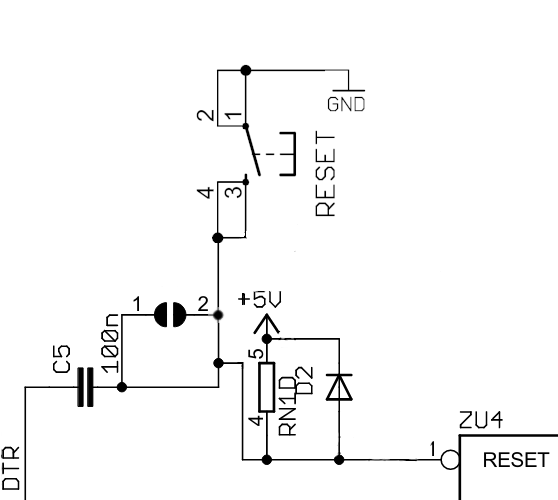
\includegraphics[width=\textwidth]{r3-rst-cap-pres-no-annotation.png}
                \begin{circuitikz}[scale=.65, american]
    
                    \draw 
                        [short, *-] (0, 0) node[label={[font=\footnotesize]left:PD7}] {} 
                        to (5, 0) node[label={[font=\footnotesize]right:\(\overline{\text{RST}}/\text{dW}\)}] {};
                    
                    \draw [short, *-] (3,0) [R] to (3,2);
                    \draw (4,0) to[short, *-] (4, 1)[D] to (4,2);
    
                    
                    \draw (3,2) to (3,2.5) to (3.5,2.5) to (3.5, 3);
                    \draw (4,2) to (4,2.5) to (3.5,2.5);
                    \draw (3,3) -- (4, 3) node[pos=.5, label=above:VCC] {};
    
                    \draw (-1.5, -1) -- (0, -1) -- (0, 1) -- (-1.5, 1);
                    \node (0) at (-0.8, 1) [label={above:\textit{Converter}}] {};
    
                    \draw (6.5, -1) -- (5, -1) -- (5, 1) -- (6.5, 1);
                    \node (0) at (5.5, 1) [label={above:\textit{target}}] {};

                    \node (0) at (2.5, -0.5) {debugWire};

    
                \end{circuitikz}
            \end{figure}
        \end{minipage}
        \note<1->{
            In figura è possibile osservare il circuito risultante.
        }
    \end{frame}
    
    \begin{frame}
        \frametitle{Server GDB e convertitore GDB-debugWire}
        \begin{itemize}
            \item[] <1-> È stato implementato un set ridotto di funzioni del protocollo GDB
            \begin{itemize}
                \item <1-> Gestione dei breakpoint
                \item <1-> Gestione della memoria SRAM (R/W)
                \item <1-> Gestione delle memorie persistenti (R/W)
            \end{itemize}
            \item[] <2-> Sono state implementate funzionalità aggiuntive quali
            \begin{itemize}
                \item <2-> Monitor debugging (RTT)
                \begin{itemize}\normalfont
                    \item<2-> Non utilizza hardware aggiuntivo
                    \item<3-> Sfrutta un buffer nella SRAM del target per la gestione del messaggio. 
                    \item<4-> Locazione del buffer nota grazie a un linker script
                \end{itemize}
            \end{itemize}
        \end{itemize}
        \note<1->{
            Sono state implementate le funzionalità presenti nel protocollo GDB le quali hanno un corrispettivo comando o sequenza di comandi debugWire.

            Alcune di esse sono la gestione dei breakpoint software e gestione delle memorie e registri in lettura e scrittura.

            Inoltre è stata implementata una funzionalità di monitor debugging attraverso la connessione debugWire, senza quindi fare affidamento su periferiche esterne per la comunicazione.
            
            Essa utilizza una libreria dedicata nel firmware del target la quale presenta un buffer nella memoria SRAM per gestire l'invio del messaggio. Questo buffer viene posizionato in un indirizzo noto (in principio alla memoria SRAM) grazie a un linker script.
        }
    \end{frame}

    \begin{frame}
        \frametitle{Monitor Debugger -- Funzionamento}
        \hspace*{-10mm}\begin{minipage}{.7\textwidth}
            \begin{itemize}
                \item[] {\color{blue} Firmware target}
                \begin{enumerate}
                    \item <1-> Scrittura del messaggio in un {\color{purple} buffer} in locazione nota
                    \item <2-> Impostazione del flag \texttt{\color{red} AVAILABLE} (locazione SRAM nota)
                    \item <3-> \texttt{asm("break");}
                \end{enumerate}
                \item[] <4-> {\color{orange} Server GDB} alla ricezione di un break
                \begin{enumerate}
                    \setcounter{enumi}{3}
                    \item <4-> Lettura flag {\color{red} \texttt{AVAILABLE}} dalla {\color{gray} SRAM} del target
                    \item <5-> Se vero
                    \begin{enumerate}
                        \item <5-> Lettura del {\color{purple} buffer} dalla SRAM
                        \item <5-> Invio del messaggio al {\color{brown} client}
                        \item <5-> Ripresa dell'esecuzione
                    \end{enumerate}
                    \item <6-> Se falso
                    \begin{enumerate}
                        \item <6-> Invio notifica di interruzione al {\color{brown} client}
                    \end{enumerate}
                \end{enumerate}
            \end{itemize}     
        \end{minipage}
        \begin{minipage}{.28\textwidth}
            \begin{figure}
                \begin{tikzpicture}[scale=.8, label distance=-2mm]

                    \draw (-0.2,-0.5) rectangle (5.2,2.2) node[pos=.08] {\hspace*{5mm}\small\textit{Target}};
                    \draw [fill=blue!50] (0,0) rectangle (2,2) node[pos=.5] {\textit{firmware}};
                    \draw [fill=green!50] (4,0) rectangle (5,0.2);
                    \draw [fill=green!50] (4,0.2) rectangle (5,0.4);
                    \draw [fill=green!50] (4,0.4) rectangle (5,1) node[pos=.5] {\tiny ...};
                    \draw [fill=purple!50] (4,1) rectangle (5,1.4) node[pos=.5] {\tiny buffer};
                    \draw [fill=red!50] (4,1.4) rectangle (5,1.7) node[pos=.5] {\tiny avail};
                    \draw [fill=gray!50] (4,1.7) rectangle (5,2)  node[pos=.5] {\tiny SRAM};
                    

                    \draw [fill=orange!50] (0,3.5) rectangle (5,4.5) node[pos=.5] {\textit{Server}};

                    \draw [fill=brown!50] (0,6) rectangle (5,7) node[pos=.5] {\textit{Client}};

                    \draw<1->[-stealth] (2,1.15) -- (4,1.15) node[pos=.25, label={above: \tiny 1}] {};
                    \draw<2->[-stealth] (2,1.5) -- (4,1.5) node[pos=.25, label={above:\tiny 2}] {};
                    \draw<3->[-stealth] (1,2) -- (1,3.5) node[pos=.5, label={right:\tiny 3}] {};
                    
                    \draw<4->[-stealth] (2,3.5) -- (4,1.6) node[pos=.5, label={above:\tiny 4}] {};

                    \draw<5->[-stealth] (1.5,3.5) -- (4,1.25) node[pos=.3, label={below:\tiny 5.1}] {};
                    \draw<5->[-stealth] (1, 4.5) -- (1,6) node[pos=.5, label={left:\tiny 5.2}] {};
                    \draw<5->[-stealth] (0.5,3.5) -- (0.5,2) node[pos=.5, label={left:\tiny 5.3}] {};

                    \draw<6->[-stealth] (1.5, 4.5) -- (1.5,6) node[pos=.5, label={right:\tiny 6.1}] {};
                \end{tikzpicture}
            \end{figure}
        \end{minipage}
        \note<1->{
            Il funzionamento della funzionalità di monitor debugging è descritto dalla sequenza seguente:
            
            Il firmware scrive nel buffer il messaggio da inviare\\
            Per segnalare la presenza del messaggio viene impostata Available.\\
            Viene eseguita l'istruzione BREAK che andrà a notificare il server dell'avvenuta interruzione\\
            Il server legge la variabile available per identificare la volontà di inviare un messaggio o il raggiungimento di un breakpoint.\\
            Se la variabile risulta vera, il server legge e inoltra il messaggio al client per poi riprendere l'esecuzione, mentre in caso contrario viene notificata l'interruzione.

            È possibile notare come il server agisca da proxy per l'evento.
        }
    \end{frame}
    
    \begin{frame}
        \frametitle{Risultati}
        \begin{minipage}{.4\textwidth}
            \begin{itemize}
                \item<1-> Debugging funzionante tramite GDB
                \item<2-> Debugging integrato nell'IDE
                \item<3-> Sistema di compilazione integrato nell'IDE
                \item <4-> Software disponibile online con licenza Open Source
            \end{itemize}
        \end{minipage}
        \begin{minipage}{.58\textwidth}
            \begin{figure}
                \includegraphics<1|handout:0>[height=.8\textheight]{../gdb-cli.png}
                \includegraphics<2|handout:0>[width=\textwidth]{vscode-dbg.png}
                \includegraphics<3|handout:0>[width=\textwidth]{vscode-cmake.png}
                \includegraphics<4>[width=\textwidth]{apache.jpg}
            \end{figure}
        \end{minipage}
        \note<1->{
            I risultati ottenuti dallo sviluppo dell'elaborato possono essere visti dall'immagine presentata.

            È stato implementato il server GDB ed è possibile effettuare il debugging.
            
            le operazioni di debugging sono state integrate nell'ide Visual Studio Code

            È stato sviluppato un sistema di compilazione e gestione delle dipendenze integrato nell'ide.

            Il software è disponibile sotto licenza open source.
        }
    \end{frame}

    \begin{frame}
        \frametitle{Conclusioni e Sviluppi futuri}
        
        \begin{itemize}
            \item[]<1-> \textbf{Conclusioni}
            \begin{itemize}
                \item <1-> Software \textbf{Open Source}
                \item <1-> \textit{Debugging} con limitato impiego di risorse
                \item <1-> Facilità d'uso
                \item <1-> Compatibilità del software su piattaforme multiple (Windows, MacOS, Linux)
            \end{itemize}
            \item[]<2-> \textbf{Sviluppi Futuri}
            \begin{itemize}
                \item<2-> Sviluppo di un hardware dedicato
                \item<2-> Migrazione a dispositivi più prestazionali
                \item<2-> Sviluppo di nuove versioni con l'ausilio del sistema attuale a fine di debug.
            \end{itemize}
        \end{itemize}
        \note<1->{
            In conclusione tutti i punti precedentemente illustrati sono stati sviluppati e correttamente implementati.

            In futuro sarà possibile sviluppare una piattaforma hardware dedicata in modo da favorire l'implementazione del firmware e sarà possibile migrare verso microcontrollori più preformanti. In particolare la scarsa quantità di memoria dell'ATMega16U2 è stata un fattore limitante delle funzionalità sviluppate.

            Sarà inoltre possibile utilizzare le funzionalità messe a disposizione da questa versione del sistema per svilupparlo.
        }
    \end{frame}

    \appendix
    \begin{frame}
        \vspace*{4cm}
        \begin{center}
            \textit{Grazie per l'attenzione}
        \end{center}
        \vspace*{2cm}
        \parbox{.85\linewidth}{
            \tiny
            \vspace*{10mm}
            {\color{unibsblue}\par\noindent\rule{\linewidth}{0.1pt}}\\
            \insertrawshotauthor\hfill
            A.A. 2021/2022\hfill
        }\hfill
        \parbox{.15\textwidth}{
            \vspace*{5mm}
            \hspace*{5mm}
            
\includegraphics[height=10mm]{logo_unibs_40.png}
        }
        \note{
            Ringraziando per l'attenzione resto a disposizione per eventuali chiarimenti.
        }
    \end{frame}
    
    \begin{frame}
        \frametitle{Livelli di comunicazione}
    
        \begin{figure}
            \begin{tikzpicture}[scale=0.80]
                \draw[fill=green!50] (0,3) rectangle (4,4) node[pos=.5] {GDB}; %GDB
                \draw[fill=yellow!50] (0,2) rectangle (4,3) node[pos=.5] {GDB proto}; %gdb_proto
                \draw[fill=red!50] (0,1) rectangle (4,2) node[pos=.5] {CDC}; %cdc
                \draw[fill=blue!50] (0,0) rectangle (4,1) node[pos=.5] {USB PHY}; %usb_phy
                
                \draw[fill=purple!50,purple!50,text=black] (5,3) rectangle (9,4) node[pos=.5] {GDB server}; %GDB_SERVER
                \draw[fill=purple!50,purple!50] (7.5,2) rectangle (9,3); 
                \draw (5,3) -- (5,4) -- (9,4) -- (9,2);
                \draw[fill=yellow] (7.75,2) rectangle (8.75,2.5) node[pos=.5] {RTT}; %RTT
        
                \draw[fill=yellow!50] (5,2) rectangle (7.5,3) node[pos=.5] {GDB proto}; %gdb_proto
                \draw[fill=red!50] (5,1) rectangle (7.5,2) node[pos=.5] {CDC}; %cdc
                \draw[fill=blue!50] (5,0) rectangle (7.5,1) node[pos=.5] {USB PHY}; %usb_phy
                \draw[fill=gray!50] (7.5,1) rectangle (9,2) node[pos=.5] {dW}; %dw
                \draw[fill=orange!50] (7.5,0) rectangle (9,1) node[pos=.5] {UART}; %uart
        
                \draw[fill=cyan!50] (10,2) rectangle (14,3) node[pos=.5] {Process}; %AVR
                \draw[fill=yellow] (13,2) rectangle (14,2.5) node[pos=.5] {RTT}; %RTT
                \draw[fill=gray!50] (10,1) rectangle (14,2) node[pos=.5] {dW}; %dw
                \draw[fill=orange!50] (10,0) rectangle (14,1) node[pos=.5] {UART (O.D.)}; %UART
        
                \draw[black, thick] (2, 0) -- (2, -0.5) -- (6.25, -0.5) -- (6.25, 0);
                \draw[black, thick] (8.5,0) -- (8.5, -0.5) -- (12, -0.5) -- (12, 0);
        
                \node (5) at (2, 4.5) {Host};
                \node (5) at (7, 4.5) {Adapter};
                \node (5) at (12, 4.5) {Tagret (AVR)};
            \end{tikzpicture}
        \end{figure}
    \end{frame}


    \begin{frame}
        \frametitle{Modifiche hardware}
        \begin{minipage}{.40\textwidth}
        %    Al fine di rendere la scheda compatibile con il protocollo debug wire:
        %    \begin{itemize}
        %        \item <1-> È stato rimosso il condensatore che isolava la connessione tra il pin dell'integrato adattatore e controllore target
        %        \item <2->  Sono state isolate alcune resistenza di pull-down
        %        \item <3->  È stato isolato il pulsante di reset
        %    \end{itemize}
        \begin{figure}
            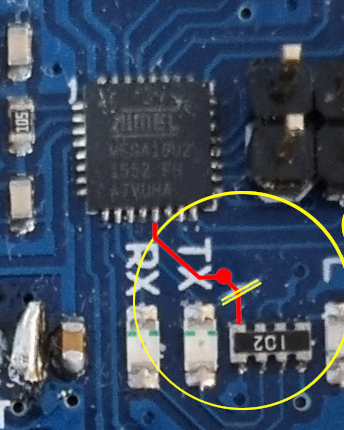
\includegraphics[width=.68\textwidth]{cut_rnd2.png}
        \end{figure}
        \end{minipage}
        \begin{minipage}{.44\textwidth}
            \begin{figure}
                \begin{minipage}{.58\textwidth}
                    \subfloat[][]{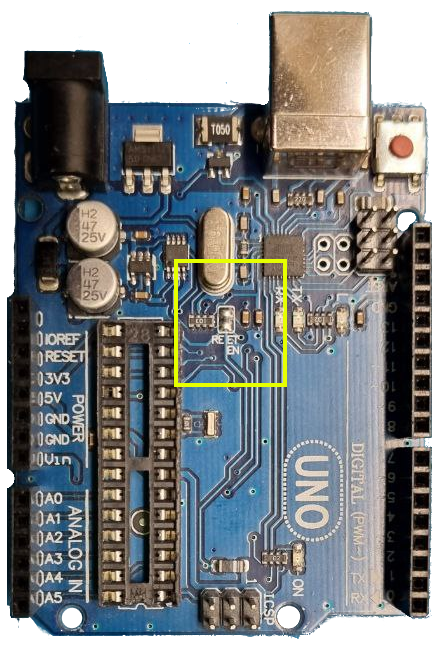
\includegraphics[width=.9\textwidth]{cap_begin.png}}
                \end{minipage}
                \begin{minipage}{.4\textwidth}
                    \subfloat[][]{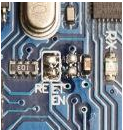
\includegraphics[width=.8\textwidth]{cap_removed.png}} \\
                    \subfloat[][]{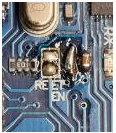
\includegraphics[width=.8\textwidth]{cap_shorted.png}}
                \end{minipage}
            \end{figure}
        \end{minipage}
    
    \end{frame}

    \begin{frame}
        \frametitle{Architettura AVR}
        \begin{minipage}{.5\textwidth}
            \begin{figure}
                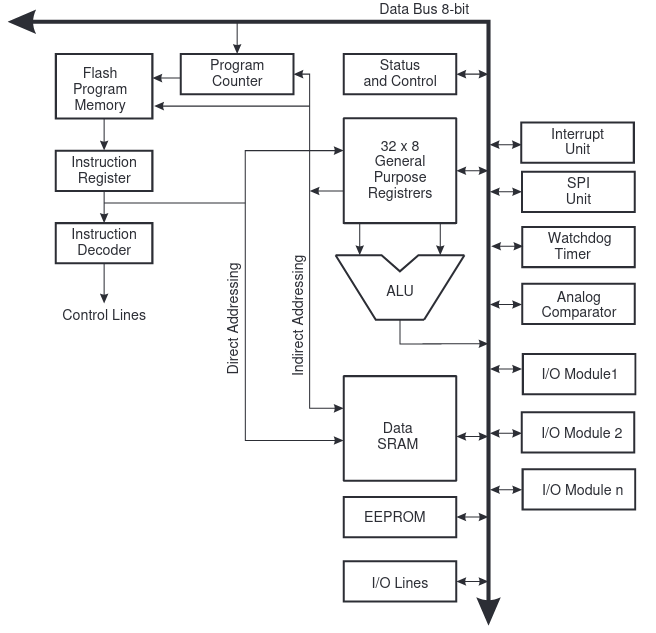
\includegraphics[width=\textwidth]{avr_arch.png}
            \end{figure}
        \end{minipage}
        \begin{minipage}{.48\textwidth}
            \begin{figure}
                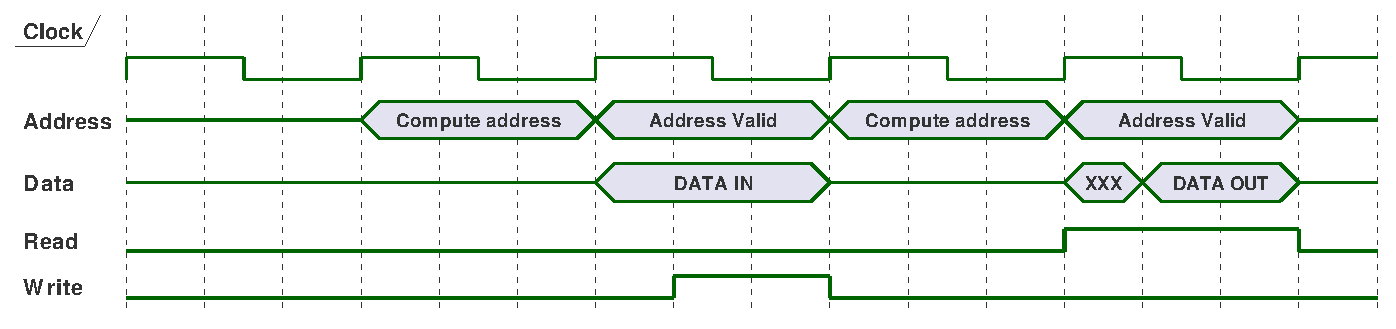
\includegraphics[width=\textwidth]{avr-sram-timings.pdf}
            \end{figure}
        \end{minipage}
    \end{frame}

\end{document}
